% This is samplepaper.tex, a sample chapter demonstrating the
% LLNCS macro package for Springer Computer Science proceedings;
% Version 2.20 of 2017/10/04
%
\documentclass[runningheads]{llncs}
%
\usepackage{mwe}
\usepackage{graphicx}
\graphicspath{{figures/}}
\usepackage{color}
\definecolor{highlight}{rgb}{1,1,0.6}
\definecolor{link}{rgb}{0.5,0.0,0.0}
\definecolor{cite}{rgb}{0.0,0.0,0.6}
\definecolor{url} {rgb}{0.3,0.0,0.3}
\definecolor{grey}{rgb}{0.3,0.3,0.3}

\usepackage[hidelinks]{hyperref}
\hypersetup{
	colorlinks,
	linkcolor={cite},
	citecolor={cite},
	urlcolor ={cite}
}

\usepackage{tabularx}
\usepackage{array}
\usepackage{booktabs} % for nice rules/lines in tables
\usepackage{arydshln} % for dashed lines in tables

\usepackage{soul} % for highlighting text
\usepackage{xspace}
\usepackage[shortcuts]{extdash}
\usepackage{relsize} % used in the \anote and \comment macros.

%% annotation commands %% 
\newcommand{\anote}[1]{{\leavevmode\smaller\itshape\color{red}\{#1\}}}
\sethlcolor{highlight}
\newcommand{\comment}[2]{\hl{#1} {{\leavevmode\smaller\color{red}\itshape\{#2\}}}}

%% PM Define authornote command for comments
\newcommand{\authornote}[1] {
	\begin{center}
		\framebox{
			{\begin{minipage}[t]{0.9\linewidth}
					\raggedright  \textbf{[PM]}~ \scriptsize #1 \normalsize
			\end{minipage}}
		}
	\end{center}
}

\newcommand*{\bibfont}{\tiny}



\newcommand{\demon}{{DEMON}}
\newcommand{\infomap}{{Infomap}}

\usepackage{amssymb}
\usepackage{bm}
\usepackage{mathtools}

% custom commands
\usepackage{rotating}
\newcolumntype{P}[1]{>{\centering\arraybackslash}p{#1}}
\newcolumntype{Y}{>{\centering\arraybackslash}X}
\usepackage{subcaption}


\begin{document}
%
\title{A customisable pipeline for continuously harvesting socially-minded Twitter users}
%
%\titlerunning{Abbreviated paper title}
% If the paper title is too long for the running head, you can set
% an abbreviated paper title here
%
\author{Flavio Primo\inst{1} \and
Paolo Missier\inst{1}\orcidID{0000-0002-0978-2446} \and
Alexander Romanovsky\inst{1}\orcidID{0000-0002-4076-3331} \and
Mickael Figueredo\inst{2} \and
Nelio Cacho\inst{2}}

%
\authorrunning{F. Primo et al.}
% First names are abbreviated in the running head.
% If there are more than two authors, 'et al.' is used.
%
\institute{Newcastle University, School of Computing \\
Science Central, Newcastle upon Tyne, UK \\
\email{\{firstname.lastname\}@ncl.ac.uk}  \and
Universidade Federal do Rio Grande do Norte \\
Natal/RN - Brasil\\
\email{neliocacho@dimap.ufrn.br}}
%
\maketitle       % typeset the header of the contribution
%
\begin{abstract}
On social media platforms and Twitter in particular, \textit{influencers} and other classes of users have been given satisfactory operational definitions in terms of Twitter content metrics.
Others, for instance \textit{online activists}, are no less important in practice but have been less precisely defined.
Supervised approaches that rely on experts' labelling of users to validate such operational definitions are often questionable, as the labels are typically biased and limited to small validation sets.
%
In contrast, we suggest a semi-supervised approach that combines two main elements. 
Firstly, we identify sets of \textit{contexts}, i.e., small but topical fragments of the network from social events or campaigns that have with a significant footprint on Twitter.
We make the hypothesis that such contexts contain meaningful signals to help us recognise activists. 
Secondly, we apply network analysis and community detection techniques to identify candidate user profiles within each context, and associate a set of quantitative Twitter-related user metrics to them.
As new online contexts occur continuously, this results in an ever-growing, feature-rich dataset of user profiles, which provides an experimental testbed. In our case, we use it to seek ranking functions that correspond to the intuitive notion of online activism.
In this paper we describe the design and implementation of the contexts harvesting and dataset population process, and we empirically demonstrate the process in action on a case study consisting of healthcare-related campaigns in the UK, showing how it supports operational definitions of online activism.

\keywords{Twitter analytics \and online user discovery \and online activists \and online influencers \and influence theories}
\end{abstract}
%

\section{Introduction}

In this paper we present a generic and customisable software framework for incrementally discovering and ranking individual profiles for classes of online users, through analysis of their social activity in micro-blogging platforms, specifically Twitter.
Practical motivation for this work comes from our ongoing effort to support health officers in tropical countries, specifically in Brazil, in their fight against airborne virus epidemics like Dengue and Zika, which are carried by mosquitoes. Help from community activists is badly needed to supplement the scarce public resources deployed on the ground. Our past work has therefore focused on identifying relevant content on Twitter that may point health authorities directly to mosquito breeding sites~\cite{Sousa2018}, as well as to users who have shown interest in those topics, i.e., by posting relevant content on Twitter~\cite{Missier2017}. 

The approach described in this paper generalises those past efforts, by attempting to discover users who demonstrate an inclination \textit{to become engaged in social issues, regardless of the specific topic}.
We refer to this class of users as \textit{activists}.
The rationale for this approach is that activists who manifest themselves online on a range of social initiatives, may be more sensitive to requests for help on specific issues. 
In the paper we experiment with healthcare-related online campaigns in the UK.

To be clear, this work is not about providing a robust definition of online activism, or to demonstrate that online activism translates into actual engagement in the ``real world''.
%
Instead, we acknowledge that the notion of activist is not as well formalised in the literature as that of, for example, \textit{influencers}. 
Thus, we have developed a generic content processing pipeline which can be customised to target specific users contexts. 
The pipeline repeatedly searches for and ranks Twitter user profiles by collecting a rich set of quantifiable network- and content-based user metrics. 
Once targeted to a specific topic, it provides a tool for exploring operational definitions of user roles, including online activism, i.e., by combining the metrics into higher level user features to be used for ranking.

Although the user harvesting pipeline described in the rest of the paper is generally applicable to the analysis of a variety of user profiles, the search for a satisfactory operational definition of online activism 
provides our main motivation. 
%
According to the Cambridge Dictionary, an \textit{activist} is ``A person who believes strongly in political or social change and takes part in activities such as public protests to try to make this happen''.
%
While activism is well-documented, e.g. in the social movement literature~\cite{doi:10.1080/14742830701497277}, and online activism is a well-known phenomenon \cite{IJoC1246}, research has been limited to the study of its broad societal impact. 
In contrast, we are interested in the fine-grained discovery of activists at the level of the single individual, that is, we seek people who feel passionate about a cause or topic, and who take action for it. 
Searching for online activists is a realistic goal, as activists presence in social media is widely acknowledged, and it is also clear that social media facilitates activists communication and organization \cite{Poell2014,Youmans2012}. 
Specific traits that characterise activists include awareness of causes and social topic and the organization of social gatherings and activities, including in emergency situations, by helping organize support efforts and diffusion of useful information.
 
\subsection{Challenges}
 
The challenges posed by the definition of online activism translate into requirements and technical challenges in systematically harvesting candidate users.
%
Firstly, the potentially more subdue nature of activists, relative to influencers, makes it particularly difficult to separate their online footprint from the background noise of general conversations.
Also, interesting activists are by their nature associated to specific topics and manifest their nature in local contexts, for instance as organisers or participants to local events. 
Finally, we expect personal engagement to be sustained over time and across multiple such contexts. 
These observations suggest that the models and algorithms developed for influencers are not immediately applicable, because they mostly operate on global networks, where less prominent users have less of a chance to emerge.
Some topic-sensitive metrics and models have been proposed to measure social influence, for example, \textit{alpha centrality}~\cite{Bonacich2001,Overbey2013} and the \textit{Information Diffusion} model~\cite{Pal2011}. Algorithms based on topic models have also been proposed to account for topic specificity~\cite{Zhao2011b}. However, these approaches are still aimed at measuring influence, not activism, and assume a one-shot discovery process, as opposed to a continuous, incremental approach.

\subsection{Approach}

To address these challenges, the approach we propose involves two strategies. 
Firstly, we identify suitable contexts that are topic-specific and limited both in time and, optionally, also in space, i.e., regional initiatives, events, or campaigns.
We then search for users only within these contexts, using a combination of network and content metrics. 
This follows the intuition that low-key users who produce weak online signal have a better chance to be discovered when the search is localised and then repeated across multiple such contexts.
By \textit{continuously discovering new contexts} and searching for users engaged in those events and campaigns, we hope to incrementally build up a users' dataset where users who appear in multiple contexts are progressively more strongly characterised.
%
Secondly, to allow experimenting with varying technical definitions of \textit{activist}, we collect a number of network-based and content-based user profile features, mostly known from the literature, and make it available for mining. Those features can be combined to generate scores that can be used to experiment with a variety of user rankings.

\subsection{ Contributions}
The paper makes the following specific contributions.
%
Firstly, we propose a data processing pipeline for harvesting Twitter content and user profiles, based on multiple limited contexts. 
The pipeline includes community detection and network analysis algorithms aimed at discovering users within such limited contexts.

Secondly, we have implemented a comprehensive set of content-based metrics that results into an ever-growing database of user profile features, which can then be used for mining purposes. 
User profiles are updated when they are repeatedly found in multiple contexts.

Lastly, for empirical evaluation of our implementation, we demonstrate an operational definition of the activist profile, defined in terms of the features available in the database, by collecting about 3,500 users  across 25 contexts in the domain of healthcare awareness campaigns in the UK during 2018. 
The application of the approach to the specific challenge of combating tropical disease epidemics in Brasil is currently in progress and is not reported in this paper.

\subsection{Related Work}

The closest body of research to this work is concerned with techniques for the discovery of online \textit{influencers} 
The characterisation of online activism given in the introduction is substantially different from that of influencers, which have received much attention in the literature.
According to ~\cite{Kardara2015}, influencers are prominent individuals with special characteristics that enable them to	affect a disproportionately large number of their peers with their actions.

A large number of metrics and techniques have been proposed to make this generic definition operational~\cite{RIQUELME2016949}. These are mostly based on metrics of network centrality, along with metrics derived from the users' online activity, i.e., number of retweets or other users' content, number of retweets of own content, and many more. 

However, most basic metrics tend to be efficient at identifying users who get great attention from their followers, such as newspapers or celebrities, but have small impact on users' actions \cite{MEEYOUNG2010}. In this way, these types of untreated metrics become inefficient to identify really active users within a topic.

In this way, algorithms to find influencers favour high visibility profiles, typically across global networks. In contrast, activists are typically low-key, less prominent users who only emerge from the crowd by signalling high levels of engagement with one or more specific topics, as opposed to being thought-leaders. 

While we believe that specific activist behavior can be characterized using some of the well-tested quantifiable metrics known from the literature cited above~\cite{RIQUELME2016949}, it should also be clear that the way such metrics are combined to identify activist profiles are not the same as for influencers. 

In \cite{MATIC2011}, a customizable valuation algorithm is created to identify influencer who are creating a revitalized level of brand awareness for companies. In this way, the raking metric is limited to one topic context. The proposed approach is cross-section variables that rate influence in social media conversations about a particular topic. The cited variables used in this study are measured using quantitative and qualitative approaches to rank the users inside a topic conversation. In the quantitative side, variables such as likes, viewers per months, post frequency the number of comments in posts are accounted. For the qualitative metrics, the number of posts positives and negatives about one topic, participation in others social medias and posts related to the main topic are considered.  The proposed approach is quite interesting to evaluate the varying degree of influence of any blogger on a particular topic. However, this approach is complex to automate due to the use of qualitative methods for the calculation of influence ranking.

Based on metrics that can be computed in an automatic way and real time, in \cite{Kardara2015} a new ranking algorithm is proposed to find local influencers on Twitter that appear within the context of a specific event being discussed, incorporating the network dynamics as the event evolves with time. However, the approach is limited to look for users using classical statics based on network created in real time. Use these ranking approach brigs the limitation to find users that are a lot of attention, but cannot create a real impact over users inside one topic.

Some approaches tries to extract the content of conversations over topics to understand the ability of a user to be influential within a topic. In \cite{Biran2012}, a classifier is trained to identify when an user is able to influencer another inside a conversation. However, in this case the necessity of create labeled data to build a machine learning classifier makes this approach impracticable in our case, which aims to be most practical possible. In addition the need to create a classifier for each topic makes the context work of this system extremely limited.


\anote{topic-specific influencers. cite \cite{Schenk2011} SCHENK 2011}\\
	
\anote{\cite{Kardara2015} KARDARA:
	Here a new ranking algorithm is proposed to find local influencers on Twitter that appear within the context of a specific event being discussed, incorporating the network dynamics as the event evolves with time. 
	Local to an event context but focus on user reputation. 
	The above techniques all attempt to define influence as
	some measurable attribute or observation in the network, such as how many times an original story appears on a website, or how centrally connected a node is within various defined modules within the networks.
	The definition used in this work for influence is “who is being listened to the most”.
	- this is not who we are looking for.
	- one single large event
	- no breakdown into communities
}\\


\anote{\cite{Bizid:2015:PUD:2808797.2809411} BIZID
	user prominence on and off topic.
	searches for specific metrics that can be computed in real time
}

%%%%%%%%%%%%%%%%%%%%%
\section{Contexts and user metrics}
%%%%%%%%%%%%%%%%%%%%%


%Two sets of criteria are used to establish relevance.
%Firstly, a context defined by a combination of spatio-temporal and keyword / hashtag constraints to describe the social topics of interest, for instance ``social health care campaigns'' or ``Zika awareness day in Rio de Janeiro''.
%%
%Secondly, a set of metrics are specified to characterise the relevance of user profiles for a specific domain, along with a user-defined function that is specific to user roles, for instance ``activist'', to compose the features into a single value, i.e., a relevance score, which can then be used to rank user profiles both within and across contexts.
%The metrics are meant to capture some operational definition of relevance for specific kinds of user roles. 

The aim of the pipeline is to repeatedly and efficiently discover user profiles from the Twitter post history within user-specified contexts,\footnote{Our plan is automate context discovery in the next phase of this work.} and use the process to grow a database of feature-rich user profiles that can be used to rank users according to user-defined relevance functions. 
The criteria used to define contexts, profile relevance functions, and associated user relevance thresholds can be configured for specific applications.

\subsection{Contexts and Context networks} \label{sec:contexts}

As described In Sec.~\ref{sec:reference}, contexts are meant to identify events or campaigns around social issues, which are characterised by temporal boundaries and by hashtags and/or keyword terms, and optionally also by spatial constraints, i.e., specified using a geographical bounding box.
These are \textit{weak} contexts, because Twitter does not natively support the notion of event or campaign (unlike, for example, Facebook, Instagram, or Meetup).
We denote a generic context as
\begin{equation}
C = \langle s, [t_1, t_2], K \rangle 
\label{eq:context}
\end{equation}
where $s$ represents the optional spatial constraint, $[t_1, t_2]$ a time interval, and $K = \{ k_1 \dots k_n\}$ is the set of terms used to filter content within the spatio-temporal boundaries.
%
$C$ defines search criteria, which produce a set $P(C)$ of posts when submitted to Twitter.
We only consider two Twitter activities: an \textit{original tweet}, or a \textit{retweet}.
Let $u(p)$ be the user who originated a tweet $p \in P(C)$.
We say that both $p$ and $u(p)$ are \textit{within context} $C$.

We also define the complement $\Tilde{P}(C)$ of $P(C)$ as the set of posts found using the same spatio-temporal constraints, but which do not contain any of the terms in $K$. More precisely, given a context $C'= \langle s, [t_1, t_2], \emptyset \rangle$ with no terms constraints, we define $\Tilde{P}(C) = P(C') \setminus P(C)$. 
We refer to these posts, and their respective users, as ``out of context $C$''.

The set of posts $P(C)$ induces a user-user social network graph $G_C = (V,E)$ where $V$ is the set of all users who have authored any $p \in P(C)$: 
$V = \{ u(p) | p \in P(C) \}$, and a weighted edge $e = \langle u_1, u_2, w \rangle$ is added to $E$ for each pair of posts $p_1, p_2$ such that $u(p_1) = u_1, u(p_2) = u_2$ and 
either (i) $p_2$ is a retweet of $p_1$, or (ii) $p_1$ contains a mention of $u_2$.
For any such edge, the weight $w$ is a count of such pairs of posts occuring in $P(C)$ for the same pair of users.

\subsection{User relevance metrics}  \label{sec:metrics}

We support a number of metrics that are generally accepted by the community as forming a core, from which many different social user roles are derived~\cite{RIQUELME2016949}. 
We distinguish amongst three types of features, which differ in the way they are computed from the raw Twitter feed:
\begin{description}
	\item[Content-based metrics] that rely solely on content and not on the user-user graph topology. These metrics are defined relative to a topic of interest, i.e., a context;
	\item[Context-independent topological metrics] that encode context-independent, long-lived relationships amongst users, i.e., follower/followee; and 
	\item[Context-specific topological metrics] that encode user relationships that occur specifically within a context.
\end{description}

All metrics are functions of a few core features that can be directly extracted from Twitter posts. 
We start with a set of features that are commonly used in the literature as a baseline.
Given a context $C$ containing user $u$, we define:
%
\begin{align*}
\mathit{R1}(u) &\text{: Number of retweets by $u$, of tweets from other in-context users;}\\
\mathit{R2}(u)&\text{: Number of unique users in $C$, who have been retweeted by $u$;}\\
\mathit{R3}(u)&\text{: Number of retweets of $u$'s tweets;}\\
\mathit{R4}(u)&\text{: Number of unique users in $C$ who retweeted $u$'s tweets;}\\
\mathit{P1}(u)&\text{: Number of original posts by $u$ within $C$;}\\
\mathit{P2}(u)&\text{: Number of web links found in original posts by $u$ within $C$;} \\
\mathit{F1}(u)& \text{: Number of followers of $u$;}\\
\mathit{F2}(u)& \text{: Number of followees of $u$}
\end{align*}
%

Note that, given $C$, we can evaluate each of the features above with respect to either $P(C)$ or  $\Tilde{P}(C)$ independently from each other, that is, we can consider a ``on-context'' and an ``off-context'' version of each feature.
%
For example, we are going to write $R1_{on}(u)$ to denote the number of context retweets and $R1_{\mathit{off}}(u)$ the number of out-of-context retweets by $u$, i.e., these are retweets that occur within $C$'s spatio-temporal boundaries, but do not contain any of the hashtags or keywords that define $C$.  
%
We similarly qualify all other features.
%
Using these core features, we have implemented the following metrics.

For \textbf{content-based metrics}, we have:
\begin{align}
\textit{Topical Focus:~\cite{Missier2017}:} ~ \mathit{TF}(u) & =  \frac{\mathit{P1}_{\mathit{on}}(u)}{\mathit{P1}_{\mathit{off}}(u) +1}    \label{eq:TF}\\
\textit{Topical Strength~\cite{Bizid2018}:} ~\mathit{TS}(u) & =	\frac{\mathit{P2}_{\mathit{on}}(u) \cdot \log(\mathit{P2}_{\mathit{on}}(u) + R3_{\mathit{on}} +1 )}{\mathit{P2}_{\mathit{off}}(u) \cdot \log(\mathit{P2}_{\mathit{off}}(u) + R3_{\mathit{off}} +1 ) + 1}   \label{eq:TS} \\
\textit{Topical Attachment~\cite{Bizid:2015,Poell2014}:} ~\mathit{TA}(u) & = \frac{\mathit{P1}_{\mathit{on}}(u) + \mathit{P2}_{\mathit{on}}(u)}{\mathit{P1}_{\mathit{off}}(u) + \mathit{P2}_{\mathit{off}}(u) +1} \label{eq:TA}
\end{align}

We implement one \textbf{Context-independent topological metric} and one \textbf{Context-specific topological metric}, both commonly used, see e.g.~\cite{RIQUELME2016949}:
\begin{align}
\textit{Follower Rank:}  \quad \mathit{FR}(u) = \frac{\mathit{F1}(u)}{\mathit{F1}(u)+\mathit{F2}(u)}   \label{eq:FR}\\
\textit{In-degree centrality:} \quad \mathit{IC}(u) = \frac{\mathit{indegree}(u)}{N-1}  \label{eq:IDC}
\end{align}
where $N$ is the number of nodes in the network induced by $C$.

Note that the metrics we have selected are a superset of those indicated in recent studies on online activism, namely \cite{Lotan2011} and \cite{Poell2014}, and thus support our empirical evaluation, described in Sec.~\ref{sec:evaluation}.


\anote{Summary of user features if space allows}

%%%%%%%%%%%%%%%%%%%%
\section{Incremental User Discovery} \label{sec:Pipeline}
%%%%%%%%%%%%%%%%%%%%

The content processing pipeline operates iteratively on a set of contexts, one at the time, that is dynamically updated at the end of each iteration, starting from an initial set of seed contexts.
The user discovery process is therefore potentially open-ended, as long as new contexts can be discovered, as explained below.
Each iteration takes a context $C$  as input, and generates a list of users who participate in $C$, along with the complete set of their features and metrics as described above. 
The users profiles are added to a database, where entries for repeat users are updated according to a user-defined function. 
The final step in the iteration involves semi-automatically discovering new contexts, thus making further iterations possible.
%
The pipeline structure and data flow are illustrated in Fig. ~\ref{fig:twitterframework}.

\begin{figure*}
	\centering
	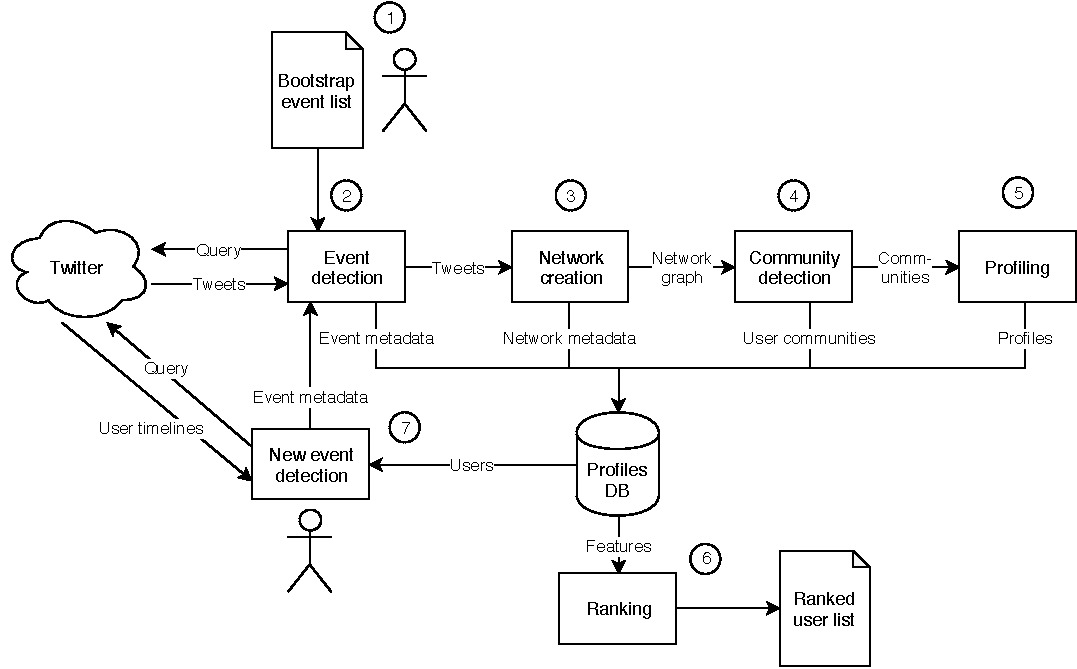
\includegraphics[width=0.7\linewidth]{figures/TwitterFramework}
	\caption{\comment{Schematic diagram of the user discovery framework }{this is a placeholder -- to be redrawn -PM }}
	\label{fig:twitterframework}
\end{figure*}

\subsection{Harvesting Content and Creating Context networks}  \label{sec:harvesting}

Firstly, all Twitter posts $P(C)$ that satisfy the criteria set in $C$ are retrieved, using either the Search or the Streaming Twitter APIs.\footnote{Repeat queries and multiple accounts are used to get around the well-known Twitter API limitations for retrieving tweets.}
%
Secondly, the context network $G_C$ is generated as defined in Sec.~\ref{sec:contexts}. To recall, this is a directed network representing retweet and/or mention interactions between pairs of users in $C$. 
The size of the network is largely determined by the nature of the context, and  ranges between 140 and 400 users (avg 254, see Table~\ref{tab:networks}).

\subsection{Community detection}  \label{sec:communities}

Next, the context network graph $G_C$  is partitioned into communities of users.
The goal of this partitioning is to further narrow the scope for the topology-sensitive metrics, namely FollowerRank (\ref{eq:FR}) and in-degree centrality (\ref{eq:IDC}), 
and thus to enable weak-signal users to emerge relative to other more globally dominant users.
%
Many different approaches have been proposed to discover virtual communities in social networks. 
We have chosen \demon~\cite{Coscia:2012:DLD:2339530.2339630} because it allows communities to overlap to a degree that is tunable, making it an ideal feature to identify users who may be active in more than one community within the same context, i.e., a social event or a campaign.

\demon identifies communities that a person belongs to with \textit{ego networks}, which consists of an individual, called the ego, and all the persons the ego has a social relationship with. 
As each ego network considers a node and its neighbours only, it provides a local method for discovering user affiliations, thus more akin to a social context.
%
It has been suggested~\cite{Arnaboldi2013} that ego networks are a useful model not only to describe social relationships amongst people offline, but also the structure of their online connections. 
Recognising that any individual may have different types of social relationships with different people (i.e., family, friends, colleagues, etc.),  \demon  naturally allows for an individual to participate in multiple communities. 

The locality principle of ego networks translates into an efficient algorithm for discovering overlapping communities in a social graph. 
Specifically, \demon operates on one node $v$ at a time in our context network $G_C$.

It applies a \textit{label propagation} algorithm to each neighbour $v'$ of $v$, as follows. First, a new label $l$, which identifies a new community, is tentatively assigned to $v'$. 
	Then, with probability $\alpha$ $v'$ changes its label to that of the majority of its own neighbours. 
	At this point, each of $v$'s neighbours has a label, which is either new or that of the majority of its own neighbours (except $v$ itself).
	$v$ is then assigned majority labels amongst those of its neighbours. 
	This determines $v$'s community. 
	When more than one label has the same count, $v$ is assigned to all of those communities.
%
As a final step, communities that overlap by more than some percentage $\epsilon $ are merged.

Note that users who do not belong to any community are discarded from the whole process.
Once communities are identified, we calculate  in-degree centrality (\ref{eq:IDC}) for each node locally, \textit{relative to their own community}.

\comment{In our evaluation we have experimented with varying values for parameters $\alpha$ an $\epsilon$...}{do we plan to say anything on how to tune them?}

\anote{what happens when nodes belong to more than one community?}

\subsection{Computing user features and ranking  \anote{PM to fix wording}}  \label{sec:features}

The next step in the process involves retrieving the core features and then the user relevance metrics as defined in Sec. ~\ref{sec:metrics}, for each user in each of the communities.
%
As this involves querying the Twitter API for many user profiles, this step hits the limitations imposed by Twitter \anote{be specific}.
To get around this problem, we have implemented a dedicated component to \textit{scrape} user information directly from their profile Web pages, namely:
\begin{itemize}
	\item personal information: the name of the user, the link to its website, the bio and the date the user joined Twitter.
	\item profile statistics: the number of tweets published, and the number of followers $F1(u)$ as well as of followees, $F2(u)$.
\end{itemize}
The latter are used directly to compute  the \textit{Follower Rank} metric (\ref{eq:FR}).
To compute the other metrics: \textit{Topical Focus} (\ref{eq:TF}), \textit{Topical Strength} (\ref{eq:TS}), \textit{Topical Attachment} \ref{eq:TA}, we further need to retrieve the entire user post history for the entire time interval defined by the context.
These posts are then separated into $P(C)$ (on-context) and $\Tilde{P}(C)$ (off-context), depending on whether they contain a hashtag related to the context or not.
Similarly, a post that contains a link is a \textit{link on-topic} that contains both a link and an hashtag related to the context, and a \textit{link off-topic} otherwise.
Note that we also calculate the number of retweets for every post, i.e., $\mathit{R1}(u)$ and $\mathit{R3}(u)$, which are required to compute \textit{Topical Strength}.

All of these features are persisted to a database which is made available for ranking purposes.
When a user already appears in the database, i.e., from previous iterations, a user-defined function can be specified to update the set of features. 
For instance, one such function could just store the average over multiple occurrences of the same user across iterations, of each of the features as well as of the metrics.
Alternatively, the database allows for the series of features values to be stored, making it possible to analyse them over time.

The main purpose of the database is to enable data analytics on a growing set of users, whose history of engagement may extend over multiple events or campaigns.
In particular, ranking is achieved by specifying a user-defined function, as described in Fig.~\ref{fig:twitterframework}, which is a function of the metrics and generates a relevance score for each user.
Note that this ``framework'' approach is consistent with the experimental nature of our search for \textit{activists}, which requires exploring a variety of ranking functions.

\subsection{Context discovery} \label{sec:context-discovery}

The final step in the iteration aims to discover new contexts. 
The idea is that, once a score function has been applied and users have been ranked, we can hope to discover new interesting keywords and hashtags in the timeline of the top-$k$ users.
Specifically,  we consider each hashtag found in the timelines, which is related to the broader topic and not yet considered in past iterations.
Each stored hashtag is then enriched with the information needed to perform a new iteration of the pipeline, namely (i) the temporal and spatial information of the context, and (ii) related hashtags.

Currently this step is only semi-automated, as it requires a human to make a judgement on the relevance of the new terms. 
One can easily imagine this step to completely automated, however, and this is one of the items for our current work.

While the process ends naturally when no new contexts are uncovered from the previous ones, the system continuously monitors the Twitter stream for recent contexts. These may typically include events that are temporally recurring, and use similar hashtags for each new edition. In this case, their relevance is assessed on the basis of their past history.


\section{Empirical Evaluation} \label{sec:evaluation}

The typical approach to identifying specific classes on online users relies on expert-generated ground truth, i.e., to determine which users belong to the desired class. 
Such approach, however, is vulnerable to  the subjectivity of the experts, whereby the evalution would  be measuring the fit of the model to the specific experts' own opinion. 
In contrast, we follow an \textit{unsupervised} approach where there is no a priori knowledge of user relevance.  
We aim to demonstrate the value of our pipeline in creating a database of online profiles, pre-selected according to specific topological properties in order to filter out background noise,  along with a community-accepted set of engineered features that are ready to be mined using any user-defined function.

Thus, our evaluation (i) shows the pipeline in action on a significant set of contexts, and (ii) demonstrates useful ranking functions that operate on the resulting database.
Specifically, we  start by manually selecting homogeneous contexts from a single social domain, namely public healthcare campaigns, to demonstrate network construction, breakdown of each  context network into communities, and harvesting of users from each community, along with their metrics.
We then provide examples of ranking functions aimed at capturing the notion of  \textit{online activists}, and we empirically validate them by inspecting the profiles of representative top-k users.

\anote{implementation:
	
	all in python. using Pandas, NetworkX, Selenium public libraries. 
	
	deployed on Azure cloud, one node with standard commodity configuration.
	
}


 \subsection{Contexts and networks}  \label{sec:contexts}
 
We have manually selected 25 contexts within the scope of health awareness campaigns in the UK, all occurring in 2018, all well-characterised using predefined hashtags.
Due to limitations imposed by Twitter on the number of posts that can be retrieved within a time interval, only $200$ tweets were retrieved from each context.
 Table~\ref{tab:contexts} lists the events along with key metrics for their corresponding user-user networks. 
To recall, \textit{assortativity} measures how frequently nodes are likely to connect to other nodes with the same degree ($>0$) or with a different degree ($<0$). 
Negative figures (mean: -0.22, std dev: 0.17) are in line with what is observed on the broader Twitter network~\cite{Fisher2017}.
%
The very small figures for density (mean: 0.004, std dev: 0.002), defined as $\frac{\#edges }{\mathit{\mathit{\#nodes}} (\mathit{\#nodes} -1)}$, suggest very few connections exist amongst users within a context. 
This makes it difficult to detect meaningful communities, as described below, thus for some context the topological metrics are measured on the entire network as opposed to within each community.
This view is also supported by the average node degree (mean: 2.04, std dev: 0.46) and the ratio of strongly connected components to the number of nodes (mean: 0.98, std. dev. 0.02).

\begin{table}
	
	\anote{content for this comes from cell [5] and cell [6] table 2 and cell [8]}
	
	\resizebox{\textwidth}{!}{
	    \newcolumntype{Y}{>{\centering\arraybackslash}X}
	
        \begin{tabularx}{\textwidth}{|X|X|X|X|X|Y|Y|Y|Y|Y|}
            \hline
            \textbf{context name} & \textbf{start date} & \textbf{end date} & \textbf{hashtags} & \textbf{assortativity} & \textbf{avg degree} & \textbf{density} & \textbf{edges} & \textbf{nodes} & \textbf{scc / nodes} \\ \hline
            16 days of action & 2018-11-25 & 2018-12-10 & \#16days, \#16daysofaction, \#16daysofactiontoolkit & -0.1 & 1.8 & 0.002 & 349 & 396 & 1.0 \\ \hline
            elf day & 2018-12-03 & 2018-12-12 & \#elfday, \#elfday2018 & -0.2 & 2.4 & 0.003 & 436 & 365 & 1.0 \\ \hline
            dry january & 2018-01-01 & 2018-01-31 & \#dryjanuary & -0.3 & 2.0 & 0.004 & 234 & 235 & 1.0 \\ \hline
            cervical cancer prevention week & 2018-01-21 & 2018-01-27 & \#cervicalcancer & -0.1 & 1.8 & 0.004 & 192 & 209 & 1.0 \\ \hline
            time to talk day & 2018-02-06 & 2018-02-07 & \#timetotalk & -0.2 & 1.7 & 0.003 & 231 & 268 & 1.0 \\ \hline
            eating disorder awareness week & 2018-02-25 & 2018-03-03 & \#edaw18, \#edaw2018, \#eatingdisordersawarenessweek, \#sockittoeatingdisorders & -0.2 & 1.9 & 0.004 & 241 & 256 & 1.0 \\ \hline
            rare disease day & 2018-02-28 & 2018-03-01 & \#rarediseaseday & -0.2 & 1.4 & 0.002 & 206 & 294 & 1.0 \\ \hline
            ovarian cancer awareness month & 2018-03-01 & 2018-03-31 & \#ovariancancer, \#ovariancancerawareness, \#ovariancancerawarenessmonth & -0.4 & 1.9 & 0.004 & 202 & 215 & 1.0 \\ \hline
            nutrition and hydration week & 2018-03-11 & 2018-03-17 & \#nutritionandhydrationweek, \#nhw2018 & -0.3 & 2.4 & 0.004 & 326 & 273 & 1.0 \\ \hline
            brain awareness week & 2018-03-11 & 2018-03-17 & \#brainawarenessweek, \#brainweek & -0.1 & 1.8 & 0.003 & 281 & 307 & 1.0 \\ \hline
            no smoking day & 2018-03-13 & 2018-03-14 & \#nosmokingday, \#smokefree & -0.3 & 1.7 & 0.003 & 219 & 254 & 1.0 \\ \hline
            epilepsy awareness purple day & 2018-03-26 & 2018-03-27 & \#purpleday, \#epilepsyawareness, \#purpleday2018 & -0.2 & 1.6 & 0.003 & 252 & 306 & 1.0 \\ \hline
            experience of care week & 2018-04-23 & 2018-04-27 & \#experienceofcareweek, \#patientexperienceweek & -0.1 & 2.2 & 0.006 & 196 & 176 & 1.0 \\ \hline
            brain injury week & 2018-05-01 & 2018-05-31 & \#braininjuryweek, \#braininjuryweek2018, \#abi2018, \#actionbraininjury2018, \#abiweek, \#hatsforheadway & -0.1 & 2.6 & 0.005 & 306 & 238 & 1.0 \\ \hline
            mental health awareness week & 2018-05-14 & 2018-05-20 & \#mentalhealthawarenessweek, \#mentalhealthawareness & -0.5 & 1.8 & 0.003 & 245 & 268 & 1.0 \\ \hline
            dementia action week & 2018-05-21 & 2018-05-31 & \#dementiaactionweek & -0.0 & 2.0 & 0.003 & 300 & 300 & 1.0 \\ \hline
            mnd awareness month & 2018-06-01 & 2018-06-30 & \#mndawareness, \#mndawarenessmonth & -0.3 & 3.3 & 0.012 & 234 & 141 & 0.9 \\ \hline
            wear purple for jia & 2018-06-01 & 2018-06-30 & \#wearpurpleforjia & -0.5 & 3.0 & 0.009 & 245 & 165 & 0.9 \\ \hline
            carers week & 2018-06-11 & 2018-06-17 & \#carersweek, \#realcarersweek, \#carersweek2018 & 0.0 & 2.1 & 0.004 & 277 & 270 & 1.0 \\ \hline
            national dementia carers & 2018-09-09 & 2018-09-10 & \#nationaldementiacarersday, \#dementiafriendly & -0.2 & 1.9 & 0.005 & 177 & 184 & 1.0 \\ \hline
            mens health week & 2018-06-11 & 2018-06-17 & \#menshealthweek & -0.2 & 1.6 & 0.003 & 214 & 264 & 1.0 \\ \hline
            stress awareness day & 2018-11-07 & 2018-11-08 & \#stressawarenessday, \#nationalstresswawarenessday, \#mentalhealthinscholls, \#listenlucy & -0.2 & 1.4 & 0.002 & 209 & 293 & 1.0 \\ \hline
            national dyslexia week & 2018-10-01 & 2018-10-07 & \#nationaldyslexiaweek, \#dyslexiaweek, \#dyslexiaawarenessweek & -0.2 & 2.1 & 0.004 & 235 & 229 & 1.0 \\ \hline
            ocd awareness week & 2018-10-07 & 2018-10-13 & \#ocdawarenessweek, \#ocdweek & -0.6 & 1.9 & 0.005 & 193 & 202 & 1.0 \\ \hline
            jeans for genes day & 2018-09-21 & 2018-09-22 & \#jeansforgenes, \#jeansforgenesday & -0.2 & 2.6 & 0.005 & 325 & 246 & 1.0 \\ \hline
        \end{tabularx}
	}
	
	\anote{add the rest of the  data from the original tables}
	\caption{List of contexts used in the experiments along with network metrics and count of \demon communities}
	\label{tab:contexts}
\end{table}	 

\subsection{Communities}  \label{sec:communities}

Next, we report on the effect of the two community detection algorithms mentioned earlier, namely \demon~and \infomap, on each of the networks. 
%
Regarding \demon, we find that, within each network, the algorithm  identifies \textit{meaningful} communities consisting of more than one single node in only 48\% of the networks, while for the remaining 52\% 
it does not detect any communities.
In this situation our pipeline creates only one community consisting of the entire network, which is used to calculate the users' in-degrees, and all users in the network are added to the database.
%
When meaningful communities are found, on the other hand, only users who belong to one of those community are added. 
These are about 6\% of the users on average, with an average of only 1.92 communities per network.
The penultimate column in Table~\ref{tab:contexts} reports the ratio of the number of communities to number of nodes in each of the networks. 
A value of zero indicates that no meaningful communities were used.
%
This approach results in 3570 users being added to the database.
The average assortativity of individual \demon~communities is slightly negative -0.28, in line with the average for their parent networks.

In contrast, the \infomap~ algorithm provides meaningful communities for all networks.
Those with fewer than 3 users are discarded, leaving  18.88 communities per network on average (as opposed to 1.92 for \demon).
The rightmost column in Table~\ref{tab:contexts} reports the number of communities normalised by the size of the network, where a community contains 8.5 users on average. 
Overall, this approach resulted in 3567 users being added to the database (on average 253 users per network).
The average assortativity across all communities is again slightly negative (-0.43).


\anote{conclude that \infomap~is preferrable and this is where the users in the database come from}

\anote{cell [10]: think about how to comment on histogram or omit altogether}


\subsection{Users discovery}  \label{sec:users}

Finally, from each context we have extracted users who are either part of a community, or in the case of non-meaningful communities, all users in the network.
Using these criteria, a total of 3567 users has been added to the database from 25 contexts.
We are interested in tracking the users' presence across more than one context, and in the specification of ranking functions that let specific user profiles emerge.

Regarding user presence, we found that there are 160 users who appear at least in two contexts. 
After community detection, only a fraction of these users survive. 
These are either users who belong to a meaningful community, or users who belong to a context network where communities could not be identified.

This filtering process results in 61 of the 160 users still seen as repeat users, while the remaining 99 are either removed altogether, or they only appear once. 
Out of these, 55 appear twice, and 2 appear three times, and 2 appear four times. 
Thus, only \hl{1.2\%} of users appear more than once when communities are considered, compared to the overall \hl{4.5\%} repeat users.
%
Table~\ref{tab:repeat-users} reports the top repeat users along with their \textit{Follower Rank}.  \anote{comment on whether these are individuals or well-known organisations}
\anote{can we sort these by no-participation and follower-rank??}
%
Fig.~\ref{fig:repeat-users-frequency} shows the number of repeat users per context. 


\begin{table}
	\centering
	\framebox{\anote{content from cell [13]} }
	
		\resizebox{\textwidth}{!}{
	
        \begin{tabularx}{\textwidth}{|X|X|X|X|X|Y|Y|}
\hline
\textbf{username} & \textbf{name} & \textbf{url} & \textbf{location} & \textbf{bio} & \textbf{follower rank} & \textbf{no participations} \\ \hline
alzheimerssoc & Alzheimer's Society & http://www.alzheimers.org.uk/ & England, Wales \& N.Ireland & We provide information and support, fund research and create lasting change for people affected by dementia. & 0.99 & 4 \\ \hline
dementiauk & Dementia UK & http://www.dementiauk.org & Aldgate, London & Dementia UK provides specialist dementia support for families through our Admiral Nurse service. We respond to messages 9-5 Monday to Friday on Twitter. & 0.98 & 4 \\ \hline
mentalhealth & Mental Health Fdn & http://www.mentalhealth.org.uk & UK & The UK's charity for everyone's mental health, promoting good mental health for all. Keep up to date with our work in Scotland by following & 0.97 & 3 \\ \hline
colesmillerllp & Coles Miller LLP & http://www.coles-miller.co.uk & Dorset & Dorset Solicitors in & 0.65 & 3 \\ \hline
rdash\_nhs & RDaSH NHS FT & http://www.rdash.nhs.uk & Doncaster & Rotherham Doncaster and South Humber NHS Foundation Trust (Monitored Mon - Fri 9am - 5pm, except Bank Holidays) & 0.88 & 2 \\ \hline
alzsocseengland & Alzheimer's Society - South East England & https://www.alzheimers.org.uk/homepage/169/our\_local\_offices &  & Alzheimer's Society ( & 0.64 & 2 \\ \hline
jeremy\_hunt & Jeremy Hunt & http://www.jeremyhunt.org &  & Foreign Secretary \& South West Surrey MP & 1.0 & 2 \\ \hline
nhsengland & NHS England & http://www.england.nhs.uk &  & Health and high quality care for all, now and for future generations. Please see our response policy: & 0.99 & 2 \\ \hline
carersuk & Carers UK & http://www.carersuk.org & United Kingdom & Caring for a relative or friend? When caring affects you and your family Carers UK is here to provide the support and advice you need. & 0.95 & 2 \\ \hline
mndassoc & MND Association & http://mndassociation.org & England, Wales \& Northern Ireland & Our vision is a world free from motor neurone disease & 0.64 & 2 \\ \hline
        \end{tabularx}
	}
	
	\caption{Top-k repeat users, amongst those identified as belonging to some community.}
	
	\label{tab:repeat-users}
\end{table}	 


\begin{figure*}
	\centering
	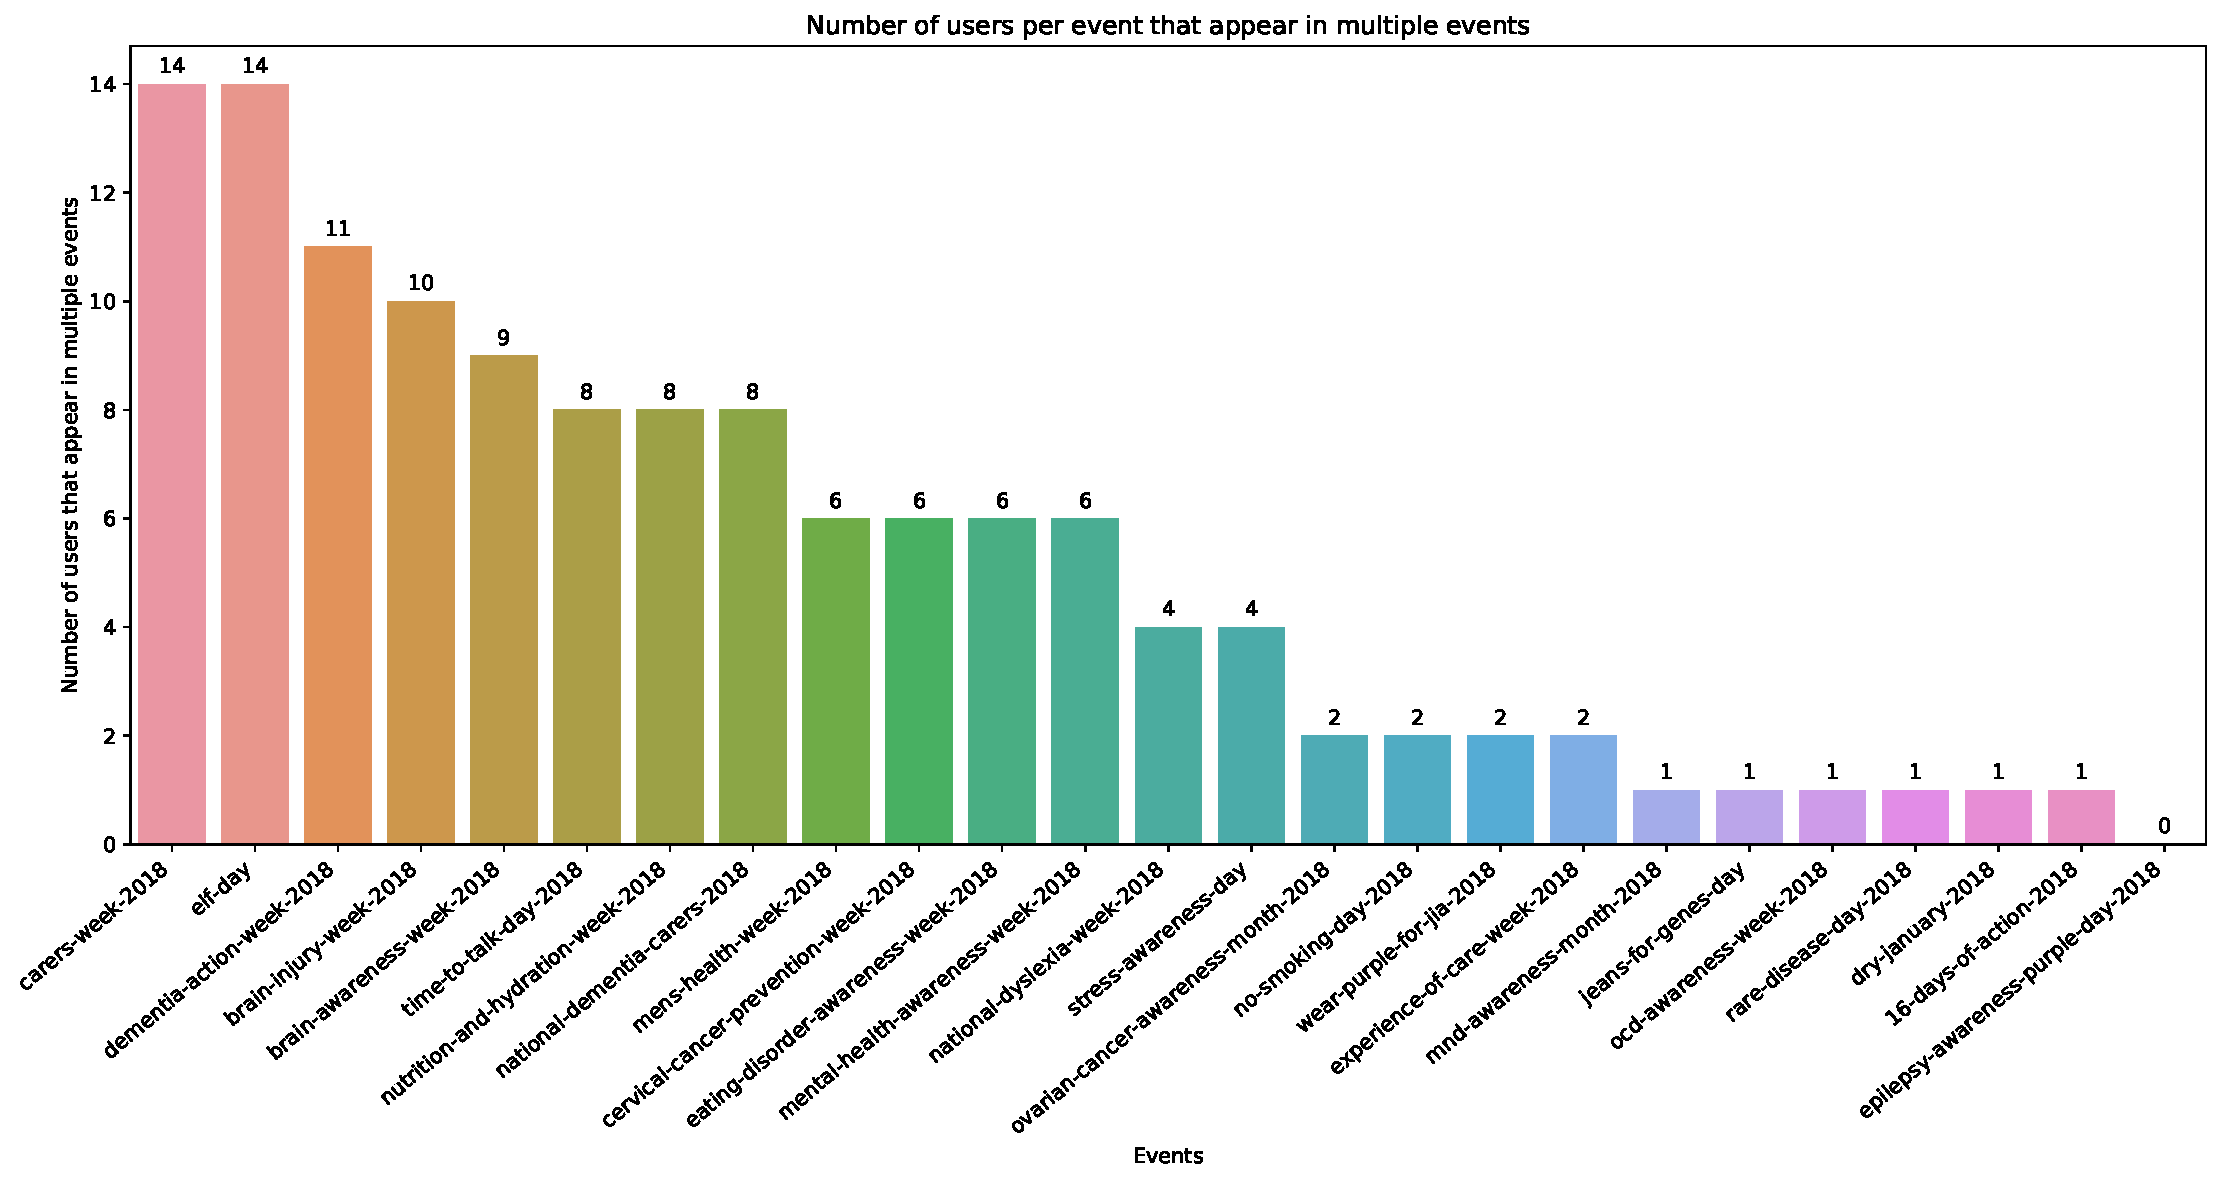
\includegraphics[width=1.2\linewidth]{figures/repeat-users-frequency}
	\caption{Number of repeat users for each context}
	\label{fig:repeat-users-frequency}
\end{figure*}

  \subsection{Users ranking} \label{sec:ranking}
  
  \anote{show the effect of one or two ranking functions and single out users that ``look like activists'' top empirically prove the point}
	
	\section{Implementation Limitations and Discussion}

	\anote{tweets harvest from the Twitter API: 200 tweets (limit is 100 but with developer account we can increase).  200 is chosen as a trade-off bet2ween the limitations on the monthly allowance (50 requests and 100/ request). we have used one single account}


\anote{network and community detection are not a bottleneck}


\anote{
	we say that events are manually identified. Sketch the events bootstrapping idea.

   also limitation from Twitter API -- 200 tweets per event.
}


 \bibliographystyle{splncs04}
 \bibliography{icwe19}

\end{document}
